\section{Resources and Process}

% \subsection{How to contribute}

The specifications of the format for a given data level defines the names and semantics of data and header fields. %Such specifications are made easy to understand. 
The specifications currently being developed can form the basis for prototypes used by data producers (mainly existing IACTs and simulated CTA data) and consumers (mainly science tools in development). We include example files and some explanations, in addition to the detailed specifications of each data level. 

The main objective of the project is to define a data format for high-level data, starting with event lists and IRFs, labeled as "data level 3" (DL3) in CTA. The first stable release (archived on Zenodo with a DOI) will be released soon.

At such an early stage there are many ways to contribute to this effort:

\begin{itemize}
\item{}Use the existing format and give feedback. Propose additions and changes.
\item{}Join the mailing list (see next section). Send an e-mail with any idea or proposal.
\item{}Create a Github account. File an issue with a correction or make a pull request proposing additions.
\end{itemize}

% No formal approval process is in place yet as this is a very recent effort.

%\subsection{Resources}
Resources:
\begin{itemize}
\item{} Mailing list for announcements and high level discussions (75 members, including people from all major gamma-ray collaborations): \\ \ogralist
\item{}Github issues and pull requests are used for detailed discussions:\\ \gadfgithub
\item{}Data format specifications in HTML and PDF format, including example files:\\ \gadfrtd
\end{itemize}

The specs are written in a markup format called "restructured text" (RST),
which gets transformed by Sphinx to HTML or PDF, the latest rendered version is always available online (see Figure~\ref{fig:webpage}).

\begin{figure}[tb]
\centerline{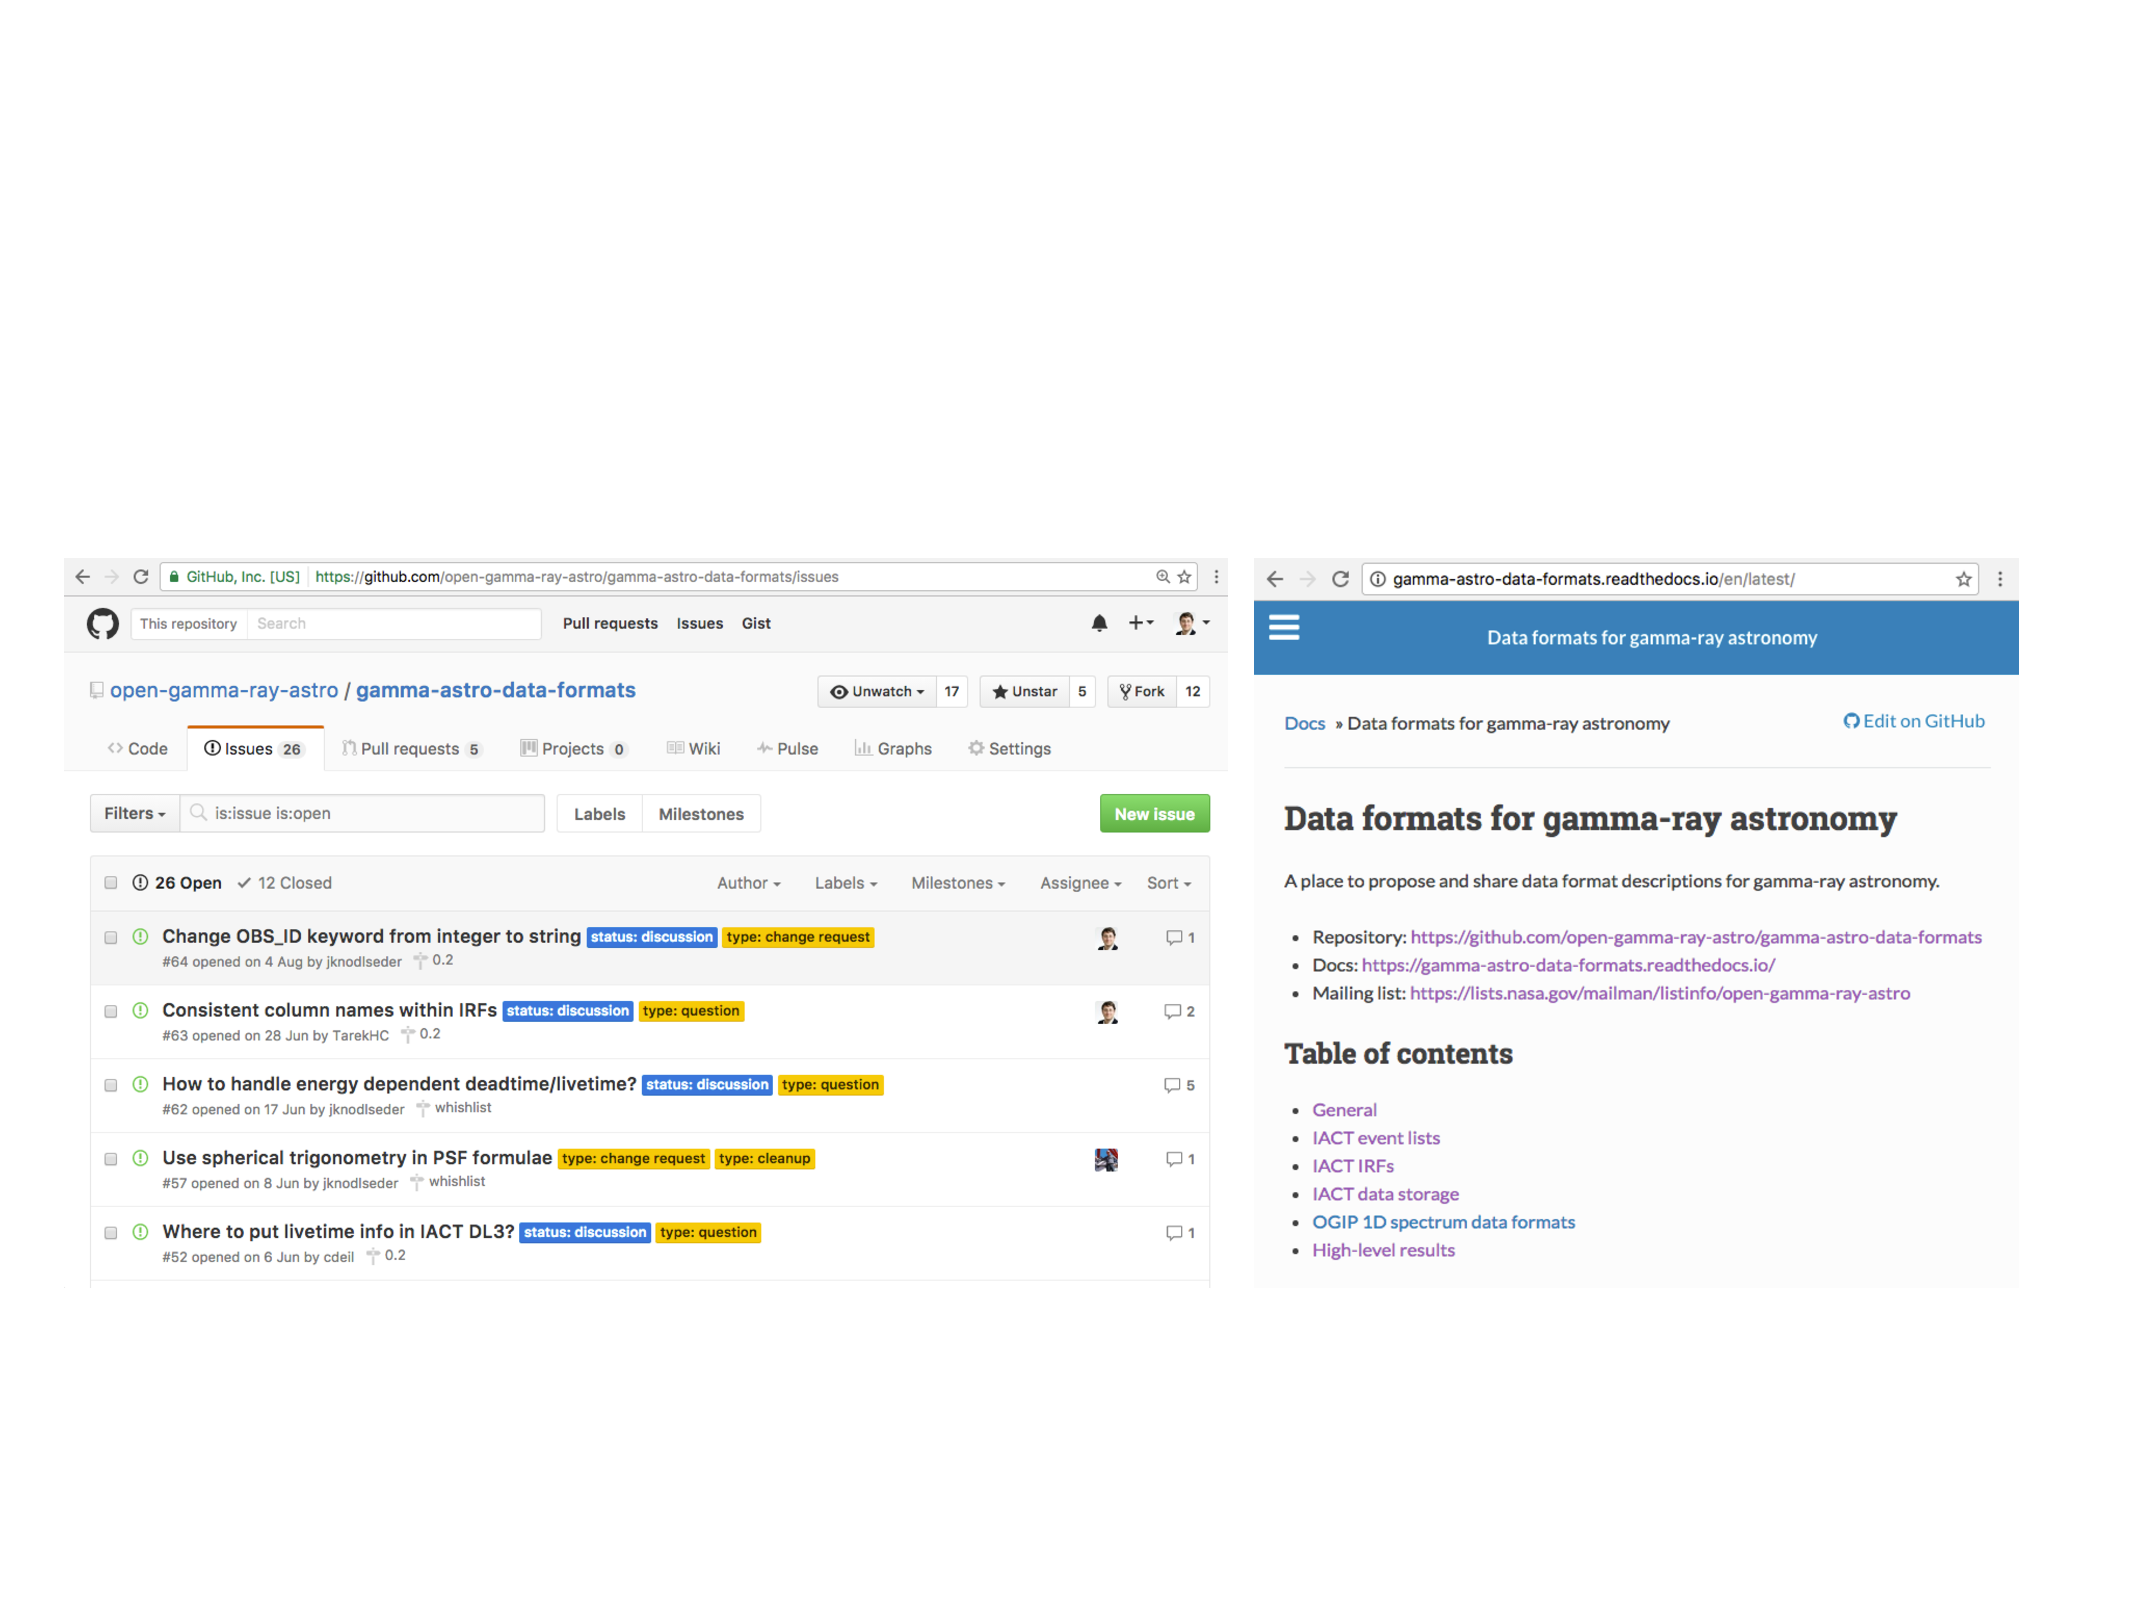
\includegraphics[width=\textwidth]{figures/webpage}}
\caption{
\emph{Left:} \texttt{gamma-astro-data-formats} Github issue tracker with ongoing discussions. \emph{Right:} latest version of the \texttt{gamma-astro-data-formats} specifications on Read the Docs (PDF and older tagged versions also available).
}
\label{fig:webpage}
\end{figure}
